%File: main.tex
\documentclass[letterpaper]{article}
\usepackage{aaai2026}
\usepackage{times}
\usepackage{helvet}
\usepackage{courier}
\usepackage[hyphens]{url}
\usepackage{graphicx}
\usepackage{natbib}
\usepackage{caption}
\usepackage{booktabs}
\usepackage{amsmath}
\usepackage{multirow}
\frenchspacing
\setlength{\pdfpagewidth}{8.5in}
\setlength{\pdfpageheight}{11in}
\setcounter{secnumdepth}{1}
\pdfinfo{/TemplateVersion (2026.1)}
\nocopyright

\title{Five Million Parameters on CIFAR-10: What Worked, What Did Not, and an Unexplained Test Gap}

\author{
  Philip Vetsas,
  Rahim Askarov
}

\affiliations{
  NYU Tandon School of Engineering, CS-GY 6953 Deep Learning, Fall 2026\\
  Team P.R.: pmv264, ra3716\\
  Code: \url{https://github.com/RoroDev2023/nyu-dl-f26-challenge}
}

\begin{document}
\maketitle

\begin{abstract}
We train a 4.88M-parameter ResNet from scratch on CIFAR-10 under a hard 5M
parameter budget and a hidden evaluation set. Our best recipe combines a long
cosine schedule, SAM, EMA, and knowledge distillation from three auxiliary
teachers, reaching 97.84\% with flip TTA (97.92\% with 10-view TTA).
The team's selected submissions scored 0.911 and 0.904 on the public leaderboard;
the private score was 0.880, placing 13th of 81 teams. The roughly ten-point gap between
validation and private accuracy is unexplained, and we report it as observed
rather than optimizing against it. We focus on measured training experiments:
the full training recipe gives the largest gains; KD adds a
smaller, schedule-confounded amount; architecture changes inside the 5M budget
give small ones; and a long list of plausible techniques did not work.
One-view AugMix was clean-neutral at 300 epochs and improved corrupted and
photometric proxies, but it was not shipped because its KD confirmation had not
finished when submissions were selected; an AugMix+JSD variant traded clean accuracy for blur
robustness and was rejected. We document the failed techniques with paired
statistics and validation curves.
\end{abstract}

\section{Introduction}

CIFAR-10~\citep{krizhevsky2009} is a small-image benchmark that modern architectures have largely
saturated: with tens of millions of parameters and long schedules, the remaining
headroom is small. The problem changes when the model must be trained from
scratch under a hard budget of five million trainable parameters, and when the
evaluation set is hidden and may not match the training distribution. Both
constraints were active in this competition. The first forces careful
architecture and optimization choices; the second makes validation accuracy an
imperfect guide and turns the leaderboard into a noisy, partially observed
signal.

We approached the problem as a two-track collaboration. One track pushed clean
accuracy through architecture search, long schedules, and knowledge distillation
(KD)~\citep{hinton2015distilling} from large teachers trained on the same data. The other track studied
robustness: it built corrupted and photometric proxy validation sets from the
training split and ran controlled augmentation ablations. The two tracks shared
one codebase, one fixed 5,000-image holdout, and one set of conventions; all numbers use
the same holdout, and the TTA/EMA protocol is stated wherever it differs.

The main result is a 4.88M-parameter student that reaches 97.84\% with
horizontal-flip test-time augmentation (TTA) and 97.92\% with 10-view TTA. The
team's selected submissions scored 0.911 and 0.904 on the public leaderboard;
the private score was 0.880, placing 13th of 81 teams. The roughly ten-point gap between our
best holdout number and the private score is the central unsolved problem of the
project. We do not have the final evaluation labels, and we do not analyze the
provided unlabeled images here, so we do not tune against the gap or claim to
explain it.

This paper makes four contributions.
\begin{itemize}
\item A strong, reproducible 4.88M-parameter ResNet~\citep{he2016deep} recipe: long cosine training~\citep{loshchilov2017sgdr}, SAM~\citep{foret2021sam},
EMA, TrivialAugment~\citep{muller2021trivial}, Cutout~\citep{devries2017cutout}, mixup/CutMix~\citep{zhang2018mixup,yun2019cutmix}, and three-teacher KD. It improves a
flip-TTA baseline from 95.42\% to 97.84\% (97.92\% with 10-view TTA) and yields
the team's 0.911 public / 0.880 private submissions.
\item A controlled account of which ingredients mattered. The training recipe gave the largest gain and KD a smaller, schedule-confounded one; architecture changes within the 5M budget gave small ones;
several plausible tricks did not pay off.
\item A clean-neutral augmentation result: one-view AugMix~\citep{hendrycks2020augmix} leaves clean accuracy
unchanged but improves a composite corruption proxy by 2.2pp and a
photographic-jitter proxy by 1.9pp, replicated across two non-KD runs, with preliminary checkpoint evaluations (epoch 200 of 300) suggesting similar gains under
distillation. A JSD variant did not preserve clean accuracy and was rejected.
\item A negative-results record. We document failed techniques with paired
statistics and validation curves: augmentation policies, late continuations,
fresh 300-epoch sweeps, test-time adaptation, TTA variants, model splitting, and
seed ensembling.
\end{itemize}

\section{Setup and Protocol}
\label{sec:setup}

\paragraph{Data and splits.}
We use the 50,000 labeled CIFAR-10 training images (10 classes, $32\times32$
RGB). A fixed stratified 5,000-image holdout (split seed 0) is used by every
student and every teacher; the remaining 45,000 images are used for training.
Teachers and students must hold out the same images, otherwise teacher
predictions on the holdout leak into the student through the soft targets. The
final full-data models are retrained on all 50,000 images once the recipe is
fixed. No external data and no pretrained weights are used.

\paragraph{Code and reproduction.}
The repository linked above contains all training code, every run's arguments and per-epoch log (\texttt{runs/}), the experiment log, the final checkpoint with its SHA-256, and \texttt{report.ipynb}. The notebook prints the parameter count (4,880,474), reloads the final checkpoint, regenerates the submitted CSV with 0 of 2,000 labels different, and recomputes the A4 holdout accuracy (97.92\%, 10-view TTA).

\paragraph{Evaluation.}
The competition metric is top-1 accuracy. The competition divides the 2,000 evaluation
images into public and private halves (1,000 each), so a public score near 90\%
has a standard error of about 1 percentage point. We use the holdout for recipe
selection and treat small public differences as noise; for full-data models
without a holdout, the public leaderboard is the final tie-breaker. Unless
stated otherwise, validation numbers use EMA weights. We report raw, EMA, flip
TTA (average of the image and its horizontal mirror), and 10-view TTA. The latter,
which we call \emph{5-crop} to match the competition codebase, averages the
softmax over a center view and four $\pm2$-pixel shifts, each with and without a
horizontal flip.

\paragraph{Paired statistics.}
Model comparisons use McNemar's exact test~\citep{mcnemar1947} on per-image correctness over the same
5,000 holdout images, with two-sided binomial $p$-values. The seed-to-seed spread on this holdout is about 0.2pp on clean data
and 0.4pp on the composite proxy, so differences of that size are treated as
noise.

\paragraph{Rules.}
The official overview asks for a modified ResNet with at most 5M trainable
parameters, trained from scratch on the permitted CIFAR-10 training data, with no
pretrained weights or external datasets. The evaluation images may not be
labeled, used for training, or used for model selection. We apply the budget to
the submitted network; the teachers are auxiliary models trained from scratch on
the same 45,000 training images (holdout excluded) and are not part of the submitted inference system. The
team submits a single network per submission. One exploratory submission used test-time BN adaptation (BN statistics re-estimated on the unlabeled evaluation images); it was rejected and is not part of the final model or the selected submissions.

\paragraph{Validation proxies.}
We build shifted validation sets from the 5,000 holdout images only. The
corruptions are Gaussian noise ($\sigma=0.05,0.10$), Gaussian blur (radius 1.0,
2.0), JPEG compression (quality 30), contrast scaling (0.7, 1.3), color
saturation (1.3), and a composite \emph{combo} (contrast 1.15, brightness 1.05,
blur 0.5, Gaussian noise $\sigma=0.02$, JPEG 75). The photographic proxies apply
per-image brightness/contrast/saturation scaling plus a small zoom and rotation:
\emph{mild} uses $\pm8\%$ brightness/contrast, $\pm12\%$ saturation, zoom 1.05 and
$\pm3^\circ$; \emph{strong} uses $\pm20\%$, $\pm30\%$, zoom 1.15 and $\pm6^\circ$.
These are label-free stress tests built from training images, not models of the
final test set.

\paragraph{Compute.}
Main runs used NYU HPC A100 nodes; ablations used A10-class cloud GPUs and a local
RTX 2070. A 4.9M student takes about 19--21s per epoch on an A10-class GPU;
three-teacher distillation takes about 59s per epoch. The longest runs (1,200
epochs on all 50k images) take about 20 hours at 59s per epoch.

\section{Methods}
\label{sec:method}

\subsection{Architectures}

\paragraph{Students.}
Our student family is a post-activation basic-block ResNet. A $3\times3$ stem
produces the first stage's channels and keeps the $32\times32$ resolution; three
stages then use 3/5/3 or 2/3/3 basic blocks, with the first block of stages 2 and
3 applying stride 2. Each block computes
$\mathrm{ReLU}(F(x)+S(x))$, where $F$ is conv--BN--ReLU--conv--BN, the last BN is
zero-initialized~\citep{goyal2017} so the residual branch starts at zero and the block starts close
to a shortcut, and $S$ is an identity or a
$1\times1$ conv--BN shortcut when the shape changes. A global average pool and a
linear layer produce the logits. The two selected presets are
\texttt{r3\_64\_3-5-3} (64/128/256 channels, 3/5/3 blocks, 4.92M parameters) and
\texttt{r3\_80\_2-3-3} (80/160/256, 2/3/3, 4.88M). A 300-epoch sweep also
evaluated \texttt{r3\_96\_2-2-2} (4.90M), \texttt{r4\_64\_3-3-2-1} (4.89M), and
\texttt{r3\_40\_8-8-8} (4.72M).

\paragraph{Design choices.}
Inside the 5M budget a stage costs roughly $B_i C_i^2$ parameters, so depth and
width trade off directly. We keep $3\times3$ convolutions ($5\times5$ costs
$2.8\times$ as much, and two stacked $3\times3$ convs already cover a
$5\times5$ receptive field), $1\times1$ projection shortcuts only where the
resolution halves (a $3\times3$ shortcut would spend budget on the pass-through
path), no max-pool in the stem so stage 1 runs at full resolution, and global
average pooling over the final $8\times8$ map. Wider stages run faster on a GPU
and give each block more features, but every block is expensive; deeper,
narrower nets are slower and become thin early (40 channels at full resolution
for \texttt{r3\_40}). The middle ground \texttt{r3\_80} (8 blocks,
80--256 channels) beat both the deeper \texttt{r3\_64} (11 blocks) and the
wider \texttt{r3\_96} (6 blocks) at 300 epochs; that mid-resolution capacity
matters most is a hypothesis from this small sweep.

\paragraph{Teachers.}
We use two WRN-28-10~\citep{zagoruyko2016wide} teachers (36.5M parameters each, seeds 0 and 1) and one
PyramidNet-110-270~\citep{han2017pyramidal} teacher with ShakeDrop~\citep{yamada2019shakedrop} (28.5M, seed 2). Teachers are trained
on the 45,000 training images for 400 epochs with the same augmentation recipe and a different seed each; the WRNs use SAM, the PyramidNet does not;
teacher size is not constrained by the 5M budget because only the student is
submitted. The teacher pool reaches 98.14\% holdout accuracy (WRN seeds 0+1); the
individual teachers reach 98.06, 98.12, and 97.64.

\subsection{Training Recipe}

All students use SGD with Nesterov momentum 0.9, batch size 128, base learning
rate 0.1, weight decay $5\times10^{-4}$ (not applied to BN affine parameters or
biases), a 5-epoch linear warmup followed by cosine decay to zero, and bf16
autocast. The default augmentation is random crop with 4-pixel padding plus
horizontal flip, TrivialAugment, Cutout 16, and per-batch mixup ($\alpha=0.2$) or
CutMix ($\alpha=1.0$) with probability 1.0. Mixing is disabled for the last 15
epochs of 300-epoch runs, 30 epochs of 600-epoch runs, 50 epochs of 1,200-epoch
runs, and 20 epochs of teacher runs. Label smoothing~\citep{szegedy2016rethinking} is 0.1 when training from hard labels and is disabled when
KD is on.

SAM with $\rho=0.05$ costs two forward/backward passes per step; the reported SAM
runs use it for the whole schedule. EMA with decay 0.999 is maintained alongside
the raw weights, and both are evaluated every epoch. The 300-epoch ablation
schedule is the shipping schedule for the augmentation comparison; the main
students use 600 or 1,200 epochs.

\subsection{Knowledge Distillation}

For ordinary KD, each teacher sees the same augmented and mixed batch as the
student (consistent teaching~\citep{beyer2022patient}), and its softened distribution is computed at temperature $T=4$. The
teacher distributions are averaged, and the student minimizes
\begin{equation}
\mathcal{L} = 0.9\,T^2\,\mathrm{KL}\!\left(\bar{p}_T \,\|\, q_T\right)
+ 0.1\,\mathrm{CE}(q, y),
\end{equation}
where $\bar{p}_T$ is the averaged teacher distribution and $q_T$ the student
distribution at the same temperature. The CE term uses the mixup/CutMix soft
targets. The two-teacher (WRN seed 0 + PyramidNet) and three-teacher runs use this loss with
\texttt{r3\_64}; the selected \texttt{r3\_80} runs use the same loss with all
three teachers.

We also implement logit-standardized KD (LS-KD)~\citep{sun2024logit}. Each teacher's logits are
z-scored per example before softening, the ensemble is averaged in that space, and
the student's logits are standardized identically. The loss is
$0.1\,\mathrm{CE} + 9\,T^2\,\mathrm{KL}$ with $T=2$. We evaluate LS-KD both as a
60-epoch continuation and as a fresh 300-epoch run.

\subsection{Augmentation Policies}

We compare five alternatives to the TrivialAugment control, all at the same
150-epoch pilot schedule (no SAM, no KD):
\begin{itemize}
\item \textbf{RandAugment}~\citep{cubuk2020randaugment}, two operations per image.
\item \textbf{AutoAugment-CIFAR}~\citep{cubuk2019autoaugment}, the learned CIFAR policy.
\item \textbf{Geometry only}: mild random affine (translation, scale, rotation).
\item \textbf{Extra affine+color}: stronger affine plus color jitter.
\item \textbf{AugMix}: the torchvision implementation with severity 3 and mixture
width 3, one view and no JSD term. This is the image-only variant; it does not add
the consistency loss.
\end{itemize}
The winner is then evaluated at 300 epochs with SAM, replicated with a second
seed, and finally tested on top of three-teacher KD. This schedule matters: the
150-epoch pilot overstates the augmentation effect because the 300-epoch control
also improves substantially.

\section{Results}
\label{sec:results}

\subsection{Main Accuracy}

Table~\ref{tab:main} summarizes the accuracy progression, and
Figure~\ref{fig:curves}(a) shows the corresponding validation curves. A plain
200-epoch student reaches 94.76\% raw (95.42\% with flip TTA). Adding the full
training recipe (300 epochs, TrivialAugment, Cutout, mixup/CutMix, SAM, EMA)
raises the flip-TTA score to 97.36\%, a gain of 1.94 points over the 95.42\%
baseline; the raw comparison (94.76 to 97.36, +2.6) mixes protocols and also
includes the 200-to-300-epoch change. Two-teacher KD at 600 epochs reaches
97.74\%. This is +0.38 over the 300-epoch no-KD run, but the schedule length
differs, so the KD effect and the schedule change are confounded. A third teacher adds only 0.02 points (97.76\%), within noise.

The wider \texttt{r3\_80} student at 600 epochs reaches 97.84\% flip and 97.92\%
5-crop; extending to 1,200 epochs (V2) gives 97.82/97.94, within noise. On the
600-epoch main path, \texttt{r3\_80} is only +0.08 over \texttt{r3\_64}
(97.84 vs.\ 97.76), also within noise; the +0.24 architecture gain is measured
at 300 epochs, not at the shipping schedule.

The full-data models have no unbiased validation score. The public leaderboard
scores are 0.904 for the two-teacher student and 0.911 for the selected
\texttt{F2s1} model (5-crop TTA; 0.903 with flip TTA only). The team's private
score is 0.880, placing 13th of 81 teams. Kaggle uses the better private score of the two
selected submissions: \texttt{F2s1} scored 0.880 private and the two-teacher student 0.876,
so the final score comes from \texttt{F2s1}. The full-data models have no holdout, so the
public LB was the final tie-breaker for the selected pair
(Figure~\ref{fig:leaderboard}).

A 4.88M student beats the 28.5M PyramidNet teacher (97.64\%) on the holdout and
comes within 0.3 points of the best two-teacher pool (98.14\%), but it does not
beat either 36.5M WRN-28-10 teacher (98.06/98.12). We interpret the result as a
well-regularized student approximating the teacher ensemble;
Figure~\ref{fig:teachers} compares them directly.

\begin{figure}[t]
\centering
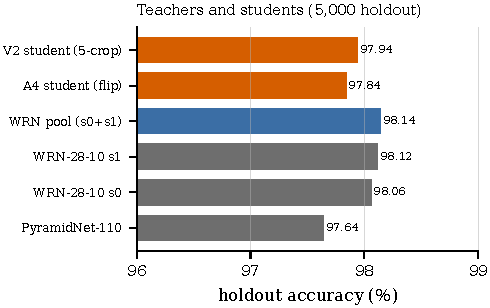
\includegraphics[width=\columnwidth]{figures/fig_teacher_student.pdf}
\caption{Teacher and student holdout accuracy. The 4.88M student is below the
best teacher pool but above the 28.5M PyramidNet teacher. A4 uses flip TTA and
V2 uses 5-crop, so the two student bars are not a controlled TTA comparison;
the x-axis starts at 96\%.}
\label{fig:teachers}
\end{figure}

\begin{table*}[t]
\centering
\small
\setlength{\tabcolsep}{4pt}
\caption{Main results on the fixed 5,000-image holdout and the leaderboard.
``Val'' is EMA + horizontal-flip TTA for every row except the baseline, which is
raw (95.42 with flip TTA); ``5-crop'' is the 10-view TTA described in
Section~\ref{sec:setup}. Full-data models have no honest validation score. Public and
private are the two 1,000-image Kaggle splits; the final score is \texttt{F2s1}'s 0.880 private (13th of 81).
The two-teacher run uses WRN seed 0 + PyramidNet.}
\label{tab:main}
\begin{tabular}{@{}lccccccc@{}}
\toprule
Run & Architecture & Params & Epochs & Val & 5-crop & Public & Private \\
\midrule
Baseline & \texttt{r3\_64\_3-5-3} & 4.92M & 200 & 94.76 & -- & -- & -- \\
All tricks, no KD & \texttt{r3\_64\_3-5-3} & 4.92M & 300 & 97.36 & -- & -- & -- \\
KD, 2 teachers & \texttt{r3\_64\_3-5-3} & 4.92M & 600 & 97.74 & -- & 0.904 & 0.876 \\
KD, 3 teachers & \texttt{r3\_64\_3-5-3} & 4.92M & 600 & 97.76 & -- & -- & -- \\
A4 (3 teachers) & \texttt{r3\_80\_2-3-3} & 4.88M & 600 & 97.84 & 97.92 & -- & -- \\
V2 (3 teachers) & \texttt{r3\_80\_2-3-3} & 4.88M & 1200 & 97.82 & 97.94 & -- & -- \\
F1 (full data) & \texttt{r3\_80\_2-3-3} & 4.88M & 600 & -- & -- & 0.898 & 0.879 \\
F2 (full data) & \texttt{r3\_80\_2-3-3} & 4.88M & 1200 & -- & -- & 0.899 & 0.879 \\
\textbf{F2s1 (selected)} & \texttt{r3\_80\_2-3-3} & 4.88M & 1200 & -- & -- & \textbf{0.911} & \textbf{0.880} \\
\bottomrule
\end{tabular}
\end{table*}

\subsection{Architecture and Distillation Ablations}

At 300 epochs and with three teachers, the architecture sweep gives 97.38\% for
\texttt{r3\_64}, 97.42\% for \texttt{r3\_96}, and 97.62\% for \texttt{r3\_80}
(Figure~\ref{fig:curves}(b)). The wider first stage is worth about 0.24 points
over the baseline shape; the deeper/narrower alternative does not help. We
therefore use \texttt{r3\_80} for the main runs. The remaining two presets
(\texttt{r4\_64} and \texttt{r3\_40}) produced logs too short for a usable curve.

The KD hyperparameter sweep is similarly flat. With \texttt{r3\_80} at 300
epochs, temperature 2 reaches 97.62\% and temperature 1 with $\alpha=1$ reaches
97.50\%, both no better than the $T=4$ baseline (97.62\%;
Figure~\ref{fig:curves}(c)). Two teachers reach 97.74\% and three reach 97.76\%
at 600 epochs; the third teacher adds 0.02 points, which is smaller than the seed
spread. We keep three teachers for the main runs because the cost is modest and
the ensemble is more stable, but we do not claim a real accuracy gain from the
third teacher.

\subsection{Robustness and Augmentation}

\paragraph{The 150-epoch pilot.}
Figure~\ref{fig:b3} compares six policies at the same cheap schedule (150
epochs, no SAM, no KD). The control (TrivialAugment) reaches 96.48\% clean TTA
and 84.32\% on the composite proxy. RandAugment (96.50/83.70) and
AutoAugment-CIFAR (96.62/83.14) are slightly better on clean data and worse on
the proxy. Geometry-only (95.98/84.96) loses 0.50 clean for 0.64 proxy.
Affine+color (95.46/84.38) loses clean accuracy without a proxy gain. One-view
AugMix is the only policy that is clean-neutral (96.52, +0.04) and substantially
better on the proxy (87.42, +3.10). The pilot motivated the full 300-epoch test,
but its effect size is inflated: the 300-epoch control also improves a lot.

\begin{figure}[t]
\centering
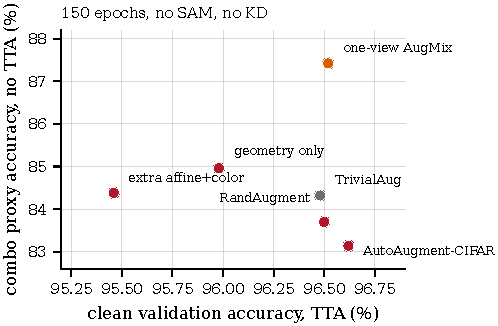
\includegraphics[width=\columnwidth]{figures/fig_b3_pilot.pdf}
\caption{Augmentation pilot at 150 epochs (no SAM, no KD). Each point is one
policy; clean points are TTA and the composite proxy is no-TTA. One-view AugMix
is the only policy that is clean-neutral and improves the proxy. The pilot
overstates the effect because the 300-epoch control is stronger.}
\label{fig:b3}
\end{figure}

\paragraph{The 300-epoch test.}
At 300 epochs with SAM, AugMix and the TrivialAugment control are identical on
clean validation (EMA 97.08\% both; flip TTA 97.06 vs.\ 97.22 in the paired evaluation, 97.04 in the run's own end-of-training log;
Figure~\ref{fig:robustness}). Under the no-TTA shifted evaluation, AugMix
improves the composite by 2.18 points (89.02 vs.\ 86.84), Gaussian noise 0.05 by
4.30, and JPEG-30 by 5.16; the matching flip-TTA paired test gives +2.28 on the
composite (89.46 vs.\ 87.18, McNemar $p=3.6\times10^{-9}$). Under flip TTA it
improves mild and strong photographic jitter by 1.10 and 1.38 points
($p\approx10^{-5}$). Geometry alone is where AugMix does nothing (+0.06 on
$\pm3$-pixel shifts), which is consistent with the gain coming from photometric
variation rather than framing. A second AugMix seed reproduces the effect (+1.80
composite; mean +1.99 across seeds) and keeps clean accuracy neutral (96.90\%).

\paragraph{Distillation.}
The provisional KD check uses the same \texttt{r3\_80} student, three teachers,
and 300 epochs, changing only \texttt{--autoaug}. In the checkpoint comparison at
epoch 200 of 300 (the archived logs stop earlier), AugMix is clean-neutral
($-0.12$, $p=0.56$) and better on the composite (+2.20,
$p=3.7\times10^{-12}$) and strong photographic jitter (+1.92,
$p=5.6\times10^{-12}$); the geometry proxy moves by +0.36 ($p=0.069$). At that
point the AugMix arm is level with the 600-epoch A4 model on the composite
(89.26 vs.\ 89.20) while still about one point behind on clean (96.86 vs.\
97.84). The effect therefore provisionally survives distillation at roughly the
same size as in the no-KD comparison. The run was interrupted and the two logs
stop at epochs 163 and 178 of 300; the comparison is provisional and was not used
for submission selection.

\paragraph{The JSD caveat.}
The B4/B5 variant is image-only, one-view AugMix without the Jensen-Shannon
consistency term. A separate 80-epoch AugMix+JSD finisher (JSD weight 12, ramped
over 10 epochs) behaved differently: it gained 2.2 points on the blur proxy
relative to the matched control but lost 0.56 points on clean validation versus
that control (96.88 vs.\ 97.44), or 0.96 versus untouched A4 (97.84). It failed our
clean-accuracy gate and was not submitted. The clean-neutral result should
therefore be read as specific to the one-view variant at the schedules we tested,
not to AugMix with JSD.

\begin{figure*}[t]
\centering
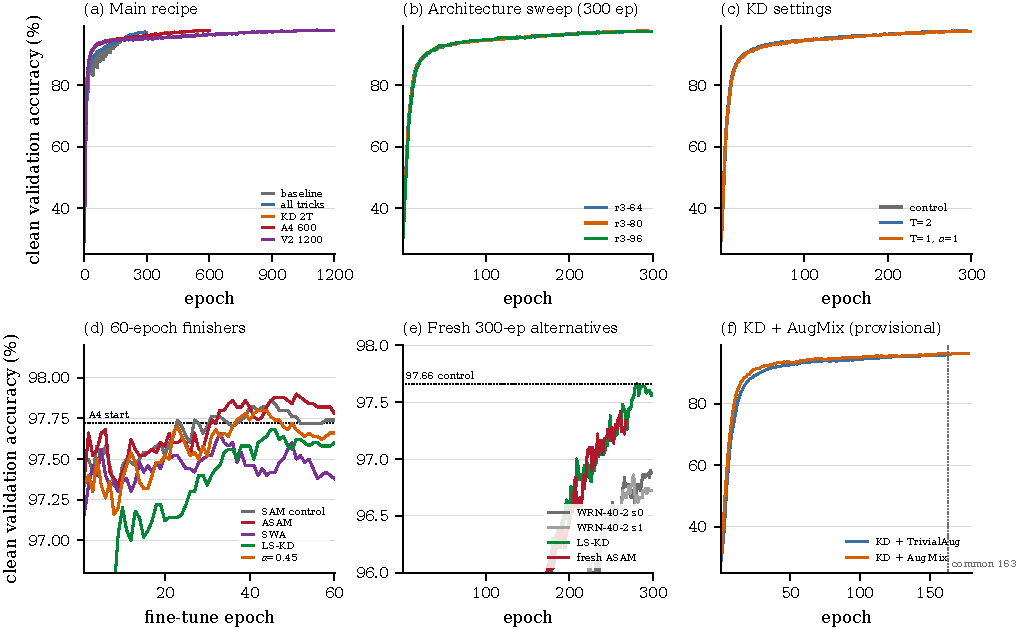
\includegraphics[width=\textwidth]{figures/fig_val_curves.pdf}
\caption{Validation curves (EMA weights unless noted, no TTA). (a) Main recipe:
baseline (raw), all tricks, two-teacher KD, A4 (600 epochs), and V2 (1,200
epochs). (b) Architecture sweep at 300 epochs. (c) KD-temperature/weight sweep.
(d) 60-epoch continuations from A4; the dotted line is the untouched A4 EMA on
the same no-TTA evaluation (97.72). The finishers stay within 0.35 points of it;
none is significant in the paired 5-crop tests (Table~\ref{tab:negative}).
(e) Fresh alternatives: the two WRN-40-2 models, LS-KD, and fresh ASAM
(stopped at epoch 268 of 300); late training is shown and none beats the
97.66\% control. (f) The provisional KD + AugMix arms; logs stop at epochs
163 and 178 of 300. Final flip/5-crop TTA numbers are in
Tables~\ref{tab:main} and~\ref{tab:negative}.}
\label{fig:curves}
\end{figure*}

\begin{figure*}[t]
\centering
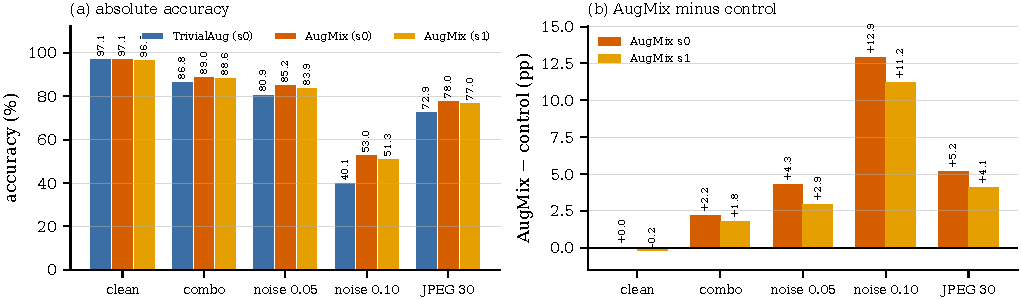
\includegraphics[width=\textwidth]{figures/fig_robustness.pdf}
\caption{B4 augmentation (EMA weights, no TTA). (a) Absolute accuracy.
(b) AugMix minus the TrivialAugment control: clean is neutral, while the
composite, noise, and JPEG proxies improve. The two seeds give +2.18 and +1.80
on the composite. These are synthetic corruptions of the labeled holdout.}
\label{fig:robustness}
\end{figure*}

\subsection{Test-Time Augmentation}

Flip TTA is the default. The 10-view 5-crop procedure adds essentially nothing
on clean data (trivial $-0.02$, AugMix $+0.10$) and is a wash overall
on the B4 arms: it helps JPEG and the composite by 0.4--1.2 points, is mixed
on noise, and hurts on zoom. Ten-view TTA requires five times as many forward passes as two-view flip TTA, or ten times as many as single-view inference. We nevertheless used
5-crop for the 0.911 submission because it exactly reproduced the team's accepted
CSV; the gain over flip is inside leaderboard noise and should not be attributed
to TTA. On the private split the selected 5-crop file scored 0.880 versus 0.883 for
flip-only TTA, which confirms this.



\subsection{The Leaderboard}

Figure~\ref{fig:leaderboard} shows every public submission. The selected
\texttt{F2s1} 5-crop run is the best at 0.911; the two-teacher student is 0.904.
Late finishers and soups built on \texttt{F2s1} score 0.908, below the untouched
model, and the exploratory test-time BN adaptation drops to 0.884. The private score is 0.880 and
the team finished 13th of 81. The gap between the 97.9\% holdout range and the
0.880 private score is the central unexplained result: we do not have the final
evaluation labels, and we do not analyze the unlabeled images here, so we cannot
identify whether the gap comes from a different capture distribution, a harder
class mix, or a smaller effective test set. We report it
as observed and do not tune against it.

\begin{figure}[t]
\centering
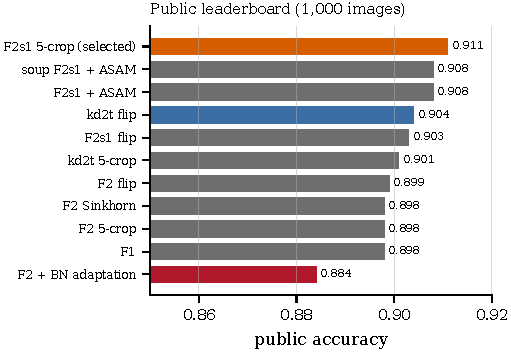
\includegraphics[width=\columnwidth]{figures/fig_leaderboard.pdf}
\caption{All public leaderboard submissions (1,000 images). The selected
\texttt{F2s1} 5-crop model is the best at 0.911; late ASAM/soup finishers sit at
0.908 and test-time BN adaptation at 0.884. The x-axis starts at 0.85; public
scores carry roughly $\pm1$pp of noise, so differences of a few images are not a
model ranking.}
\label{fig:leaderboard}
\end{figure}

\section{What Did Not Work}
\label{sec:negative}

The competition rewarded clean accuracy, but a large fraction of our experiments
did not improve it. We report them here because the failure pattern is
informative: several techniques that are strong in the literature are neutral or
negative at this budget and schedule, and several apparent gains disappear under
a matched control. Table~\ref{tab:negative} summarizes the results; the text gives
the context.



\begin{table*}[t]
\centering
\footnotesize
\setlength{\tabcolsep}{2.5pt}
\caption{Techniques that did not pay off. $\Delta$ is in percentage points on the
5,000-image holdout unless the row uses the public leaderboard. Paired McNemar
$p$-values are shown where recorded; ``--'' means no paired test was logged.
Pilot numbers are clean TTA / combo; the B4 comparison is in
Figure~\ref{fig:robustness} and Section~\ref{sec:results}.}
\label{tab:negative}
\begin{tabular}{@{}p{0.17\textwidth}p{0.42\textwidth}rrp{0.17\textwidth}@{}}
\toprule
Technique & Matched comparison & $\Delta$ & $p$ & Verdict \\
\midrule
\multicolumn{5}{@{}l}{\emph{Augmentation (150-epoch pilot, clean TTA / combo)}}\\
RandAugment & 96.50 / 83.70 vs.\ 96.48 / 84.32 & $+0.02$ / $-0.62$ & -- & worse proxy \\
AutoAugment-CIFAR & 96.62 / 83.14 vs.\ control & $+0.14$ / $-1.18$ & -- & worse proxy \\
Geometry only & 95.98 / 84.96 vs.\ control & $-0.50$ / $+0.64$ & -- & clean drop \\
Extra affine+color & 95.46 / 84.38 vs.\ control & $-1.02$ / $+0.06$ & -- & clean drop \\
\midrule
\multicolumn{5}{@{}l}{\emph{Optimization and KD}}\\
ASAM continuation & 98.00 vs.\ 97.82 (SAM) & $+0.18$ & 0.049 & no significant gain over A4 \\
LS-KD (300 ep) & 97.50 vs.\ 97.62 (flip) & $-0.12$ & -- & no gain; lower NLL \\
WRN-40-2 pair & 97.26 vs.\ 97.62 (one \texttt{r3\_80}) & $-0.36$ & -- & loses \\
\midrule
\multicolumn{5}{@{}l}{\emph{Inference and adaptation}}\\
5-crop TTA & 97.20 vs.\ 97.22 (trivial); 97.16 vs.\ 97.06 (AugMix) & $-0.02$ / $+0.10$ & 1.0 / 0.33 & wash \\
Test-time BN & 0.884 vs.\ 0.899 public & $-1.5$ & -- & hurts \\
Sinkhorn balance & 0.898 vs.\ 0.899 public & $-0.1$ & -- & no gain \\
2-seed ensemble & +0.34 combo, +0.44 strong-photo & $+0.3$--$0.4$ & 0.15 / 0.02 & inside noise \\
Train-split BN & 97.08 / 97.20 vs.\ 97.84 / 97.82 (flip) & $-0.76$ / $-0.62$ & -- & hurts \\
\bottomrule
\end{tabular}
\end{table*}

\paragraph{Augmentation.}
RandAugment and AutoAugment-CIFAR are clean-neutral or slightly positive, but both
make the composite proxy worse than the TrivialAugment control. Geometry-only
augmentation trades 0.50 clean points for 0.64 proxy points, which fails our
clean-drop budget; affine+color loses 1.02 clean points with no proxy gain.
AugMix is the exception and is discussed in Section~\ref{sec:results}.

\paragraph{ASAM and SWA.}
ASAM~\citep{kwon2021asam} and SWA~\citep{izmailov2018swa} were tested as late continuations.
Figure~\ref{fig:curves}(d) shows the five 60-epoch continuations from A4; none
produces a significant gain over the untouched start. A 60-epoch ASAM continuation beats the matched SAM
continuation by 0.18 points (98.00 vs.\ 97.82, $p=0.049$; five finishers
were compared, so this uncorrected $p$ is exploratory), but it does not beat
the untouched A4 start point (97.92; $+0.08$, $p=0.50$). The confirm run from the
two-teacher student moves by +1 image against its SAM control and +2 against the
untouched model ($p=0.83$). ASAM is better than SAM for
this late continuation, but the continuation itself gives no statistically significant gain over the untouched model.
SWA is neutral under 5-crop (97.80 vs.\ 97.82) but is 0.34 lower on the
no-TTA curve. A fresh ASAM run (stopped at 268 of 300 epochs) changes one image
(97.64 vs.\ 97.62); applying the 60-epoch ASAM finish to F2s1 changes 33/2,000
test labels and scores 0.908 public versus 0.911 for the untouched model; the
corresponding weight soup~\citep{wortsman2022soups} also scores 0.908 (Figure~\ref{fig:leaderboard}). No
completed fresh 1,200-epoch ASAM/SWA run exists; F1200\_asam was stopped at
epoch 250.

\paragraph{LS-KD.}
Logit-standardized KD reduced validation NLL without improving top-1 accuracy in our hands. The continuation matches ordinary KD under 5-crop (97.76 vs.\ 97.82, within
noise). The fresh run reaches 97.62 5-crop / 97.50 flip, while the archived
ordinary-KD baseline is 97.62 flip; the protocols differ, so we do not claim an
accuracy gain. Validation NLL is lower in both cases (0.086 for the continuation
and 0.092 fresh, versus about 0.15). We did not measure calibration directly; for top-1 accuracy it is a wash.

\paragraph{Splitting the budget.}
Two WRN-40-2 models (2.24M each, 4.49M together) reach 97.10 and 97.08
individually; their equal-probability ensemble reaches 97.26. The ensemble gains
only +0.16 over one WRN and remains 0.36 below a single 4.88M \texttt{r3\_80}
(97.62). With this recipe, splitting the parameter budget into two smaller models
is worse than spending it on one. The pair's errors are also highly correlated
(111 images wrong in both; Jaccard overlap 0.61), so the ensemble has little
diversity to exploit.

\paragraph{TTA, adaptation, and ensembling.}
The 10-view TTA is a wash on clean data and only helps on JPEG/composite proxies;
flip TTA captures most of it. Test-time BN adaptation, which recomputes BN
statistics on the evaluation images, drops the public score from 0.899 to 0.884
(one exploratory submission, rejected).
Sinkhorn class balancing~\citep{cuturi2013sinkhorn} is neutral (0.898 vs.\ 0.899). A two-seed AugMix
ensemble gains +0.34 on the composite ($p=0.15$) and +0.44 on strong photographic
jitter ($p=0.02$), but the composite gain is not significant and both are inside
the public-LB noise; we did not use an ensemble for the final submission.
Train-split BN recalibration (recomputing BN on clean training images) hurts
under the same flip protocol: 97.08 vs.\ 97.84 for A4 and 97.20 vs.\ 97.82 for
V2. The augmentation-trained BN statistics are better on our holdout; we do not
claim that this transfers to the hidden set.

\paragraph{Fresh 300-epoch sweep.}
Figure~\ref{fig:curves}(e) shows the fresh alternatives. A matched
300-epoch sweep found no gain from extra regularization or a different KD weight:
two-teacher KD with the two WRNs only is neutral (97.66), KD $\alpha=0.45$ loses 11 images, and
stochastic depth~\citep{huang2016deep} 0.1 loses 18 (97.30 vs.\ 97.66, $p=0.005$).



\paragraph{What we did not test.}
DKD, structural teacher pruning, and completed fresh 1,200-epoch ASAM/SWA/LS-KD
runs were left untested. An SE run was launched but never scored. These are the
most promising follow-ups but did not fit the compute budget.

\section{Discussion and Limitations}
\label{sec:discussion}

\paragraph{What produced the accuracy.}
The largest single jump came from the training recipe rather than the
architecture: the 95.42\% flip-TTA baseline became 97.36\% with long training,
TrivialAugment, Cutout, mixup/CutMix, SAM, and EMA. KD at 600 epochs reaches
97.74\%, but that comparison also changes the schedule, so it is an upper bound
on the KD effect. The wider student adds 0.24 points at 300 epochs but only 0.08
on the 600-epoch main path, within noise. The 4.88M student ends up better than
the 28.5M PyramidNet teacher (97.64\%) and within 0.3 points of the two-teacher
pool (98.14\%), but it does not beat either 36.5M WRN-28-10 teacher
(98.06/98.12). Architecture search inside the 5M budget was secondary.

\paragraph{The unexplained gap.}
A4 reaches 97.92\% with 5-crop and V2 reaches 97.94\%, a 0.02 difference that is
not meaningful; we treat the 97.9\% range as the headline holdout result. The
selected submissions scored 0.911 and 0.904 public, and the team's private score
was 0.880, 13th of 81. The private score is roughly ten points below the holdout
range, and the gap between the best public score (0.911) and the private score
(0.880) is 3.1 points. Because the public and private halves are 1,000 images
each, part of that difference is sampling noise; the rest could be a harder
private subset, a different capture distribution, or both. We do not have the
final evaluation labels, and we do not analyze the provided unlabeled images
here, so we cannot separate these causes.

\paragraph{Why one-view AugMix was not shipped.}
One-view AugMix is the one robustness intervention that survived every check we
ran: it is clean-neutral at 300 epochs, improves the composite by 2.2 points,
improves photographic jitter by 1.1--1.9 points, replicates across seeds, and
keeps its effect under three-teacher KD. It was still not in the final submission.
The KD confirmation had not finished when the team selected its submissions; its
logs stop at epoch 178/300, and the full-data 1,200-epoch AugMix run was never
trained. Given that the final private gap is unexplained, we cannot claim that
shipping AugMix would have improved the score. The honest conclusion is that it
was the best-supported robustness candidate we had, and the submission schedule
did not allow us to test it at the shipping scale.

\paragraph{Limitations.}
Most comparisons use a single seed; the exceptions are the two AugMix seeds and
the ASAM confirm. The holdout is 5,000 images, so the seed-to-seed spread is
0.2--0.4 points and small differences should not be over-interpreted. The B5 KD
comparison is provisional at 200/300 epochs and was interrupted twice; its
partial curves are in Figure~\ref{fig:curves}(f). The proxies are synthetic and label-free stress tests, not models of the final
shift. Both leaderboards are 1,000 images, so they are noisy. We have no completed fresh 1,200-epoch ASAM,
SWA, or LS-KD run (F1200\_asam stopped at epoch 250), and we did not test DKD or
structural teacher pruning. Finally, the full-data models have no unbiased
validation score, so the final selection relies on the holdout models and, for
the full-data pair, the public leaderboard.

\paragraph{What we would do differently.}
First, ablate augmentation at the shipping schedule: the 150-epoch pilot
overstated AugMix's effect because the 300-epoch control improved so much. Second, keep per-epoch logs for every run in the repository; several
curves in this paper are missing because the logs stayed on a cluster or a cloud
volume. Third, complete the KD robustness run before submission selection, so
that a clean-neutral augmentation has a chance to ship. Fourth, run the main
comparisons with at least two seeds; the single-seed spread is large enough to
swallow several of the effects we measured.

\section{Conclusion}
\label{sec:conclusion}

Our 4.88M-parameter ResNet reaches 97.84\% with flip TTA (97.92\% with 10-view
TTA). The selected submissions scored 0.911 and 0.904 public; the private score
was 0.880, 13th of 81 teams. The recipe---long cosine training, SAM, EMA,
TrivialAugment, Cutout, mixup/CutMix, and three-teacher KD---is strong at this
budget: the student beats the 28.5M PyramidNet teacher, though not the 36.5M
WRNs.

The project also produced a negative-results catalog. RandAugment,
AutoAugment-CIFAR, geometry-only and affine+color augmentation, ASAM/SWA
fine-tuning, logit-standardized KD, a two-model split, multi-crop TTA, test-time
BN adaptation, Sinkhorn balancing, and seed ensembling produced no significant or
shipping gain. One-view AugMix was the exception: clean-neutral and better on
corrupted and photometric proxies, but not shipped because its KD confirmation
had not finished when submissions were selected.

The roughly ten-point gap between clean validation and the private leaderboard is
unexplained: we lack final labels and do not analyze the unlabeled images here.

\begin{thebibliography}{}
\footnotesize
\setlength{\itemsep}{0pt}
\bibitem[Beyer et~al.(2022)]{beyer2022patient} Beyer, L., et~al. 2022. Knowledge distillation: A good teacher is patient and consistent. In \emph{CVPR}.
\bibitem[Cubuk et~al.(2019)]{cubuk2019autoaugment} Cubuk, E.~D.; Zoph, B.; Man\'e, D.; Vasudevan, V.; and Le, Q.~V. 2019. AutoAugment: Learning augmentation strategies from data. In \emph{CVPR}.
\bibitem[Cubuk et~al.(2020)]{cubuk2020randaugment} Cubuk, E.~D.; Zoph, B.; Shlens, J.; and Le, Q.~V. 2020. RandAugment: Practical automated data augmentation with a reduced search space. In \emph{CVPR Workshops}.
\bibitem[Cuturi(2013)]{cuturi2013sinkhorn} Cuturi, M. 2013. Sinkhorn distances: Lightspeed computation of optimal transport. In \emph{NeurIPS}.
\bibitem[DeVries and Taylor(2017)]{devries2017cutout} DeVries, T.; and Taylor, G.~W. 2017. Improved regularization of convolutional neural networks with Cutout. arXiv:1708.04552.
\bibitem[Foret et~al.(2021)]{foret2021sam} Foret, P.; Kleiner, A.; Mobahi, H.; and Neyshabur, B. 2021. Sharpness-aware minimization for efficiently improving generalization. In \emph{ICLR}.
\bibitem[Goyal et~al.(2017)]{goyal2017} Goyal, P., et~al. 2017. Accurate, large minibatch SGD: Training ImageNet in 1 hour. arXiv:1706.02677.
\bibitem[Han, Kim, and Kim(2017)]{han2017pyramidal} Han, D.; Kim, J.; and Kim, J. 2017. Deep pyramidal residual networks. In \emph{CVPR}.
\bibitem[He et~al.(2016)]{he2016deep} He, K.; Zhang, X.; Ren, S.; and Sun, J. 2016. Deep residual learning for image recognition. In \emph{CVPR}.
\bibitem[Hendrycks et~al.(2020)]{hendrycks2020augmix} Hendrycks, D., et~al. 2020. AugMix: A simple data processing method to improve robustness and uncertainty. In \emph{ICLR}.
\bibitem[Hinton, Vinyals, and Dean(2015)]{hinton2015distilling} Hinton, G.; Vinyals, O.; and Dean, J. 2015. Distilling the knowledge in a neural network. arXiv:1503.02531.
\bibitem[Huang et~al.(2016)]{huang2016deep} Huang, G.; Sun, Y.; Liu, Z.; Sedra, D.; and Weinberger, K.~Q. 2016. Deep networks with stochastic depth. In \emph{ECCV}.
\bibitem[Izmailov et~al.(2018)]{izmailov2018swa} Izmailov, P.; Podoprikhin, D.; Garipov, T.; Vetrov, D.; and Wilson, A.~G. 2018. Averaging weights leads to wider optima and better generalization. In \emph{UAI}.
\bibitem[Krizhevsky(2009)]{krizhevsky2009} Krizhevsky, A. 2009. Learning multiple layers of features from tiny images. Technical report, University of Toronto.
\bibitem[Kwon et~al.(2021)]{kwon2021asam} Kwon, J.; Kim, J.; Park, H.; and Choi, I.~K. 2021. ASAM: Adaptive sharpness-aware minimization for scale-invariant learning of deep neural networks. In \emph{ICML}.
\bibitem[Loshchilov and Hutter(2017)]{loshchilov2017sgdr} Loshchilov, I.; and Hutter, F. 2017. SGDR: Stochastic gradient descent with warm restarts. In \emph{ICLR}.
\bibitem[McNemar(1947)]{mcnemar1947} McNemar, Q. 1947. Note on the sampling error of the difference between correlated proportions or percentages. \emph{Psychometrika} 12(2): 153--157.
\bibitem[M\"uller and Hutter(2021)]{muller2021trivial} M\"uller, S.~G.; and Hutter, F. 2021. TrivialAugment: Tuning-free yet state-of-the-art data augmentation. In \emph{ICCV}.
\bibitem[Sun et~al.(2024)]{sun2024logit} Sun, S.; Ren, W.; Li, J.; Wang, R.; and Cao, X. 2024. Logit standardization in knowledge distillation. In \emph{CVPR}.
\bibitem[Szegedy et~al.(2016)]{szegedy2016rethinking} Szegedy, C.; Vanhoucke, V.; Ioffe, S.; Shlens, J.; and Wojna, Z. 2016. Rethinking the Inception architecture for computer vision. In \emph{CVPR}.
\bibitem[Wortsman et~al.(2022)]{wortsman2022soups} Wortsman, M., et~al. 2022. Model soups: Averaging weights of multiple fine-tuned models improves accuracy without increasing inference time. In \emph{ICML}.
\bibitem[Yamada et~al.(2019)]{yamada2019shakedrop} Yamada, Y.; Iwamura, M.; Akiba, T.; and Kise, K. 2019. ShakeDrop regularization for deep residual learning. \emph{IEEE Access} 7: 186126--186136.
\bibitem[Yun et~al.(2019)]{yun2019cutmix} Yun, S.; Han, D.; Oh, S.~J.; Chun, S.; Choe, J.; and Yoo, Y. 2019. CutMix: Regularization strategy to train strong classifiers with localizable features. In \emph{ICCV}.
\bibitem[Zagoruyko and Komodakis(2016)]{zagoruyko2016wide} Zagoruyko, S.; and Komodakis, N. 2016. Wide residual networks. In \emph{BMVC}.
\bibitem[Zhang et~al.(2018)]{zhang2018mixup} Zhang, H.; Cisse, M.; Dauphin, Y.~N.; and Lopez-Paz, D. 2018. mixup: Beyond empirical risk minimization. In \emph{ICLR}.
\end{thebibliography}


\end{document}
